\documentclass[a4paper]{report}

\usepackage{../mathstemplate}

\date{IV семестр, весна 2024 г.}
\title{Алгебра. Неофициальный конспект}
\author{Лектор: Алексей Владимирович Степанов\\ Конспектировал Леонид Данилевич}

\begin{document}
    \shorthandoff{"}
    \maketitle
    \tableofcontents
    \newpage
    \setcounter{lection}{0}


    \chapter{Гомологическая алгебра}
    \newlection{12 февраля 2024 г.}
    \section{Абелевы категории}
    Напомним некоторые определения из предыдущей лекции.
    \definition[Предаддитивная категория $\cat{A}$]{
        $\forall A, B \in \cat{A}: \Mor_{\cat{A}}(A, B)$ образует абелеву группу, и везде, где определена, выполнена дистрибутивность: \[\alpha(\beta+\gamma) = \alpha\beta + \alpha\gamma \qquad (\beta + \gamma)\alpha = \beta\alpha + \gamma\alpha\]
    }
    \definition[Бипроизведение]{ Такая диаграмма, что
    % https://q.uiver.app/#q=WzAsMyxbMSwwLCJDIl0sWzAsMCwiQSJdLFsyLDAsIkIiXSxbMSwwLCJcXGlvdGFfMSIsMix7Im9mZnNldCI6MX1dLFswLDEsIlxccGlfMSIsMix7Im9mZnNldCI6MX1dLFswLDIsIlxccGlfMiIsMCx7Im9mZnNldCI6LTF9XSxbMiwwLCJcXGlvdGFfMiIsMCx7Im9mZnNldCI6LTF9XV0=
        \[\begin{tikzcd}[ampersand replacement=\&]
              A \& C \& B
              \arrow["{\iota_1}"', shift right, from=1-1, to=1-2]
              \arrow["{\pi_1}"', shift right, from=1-2, to=1-1]
              \arrow["{\pi_2}", shift left, from=1-2, to=1-3]
              \arrow["{\iota_2}", shift left, from=1-3, to=1-2]
        \end{tikzcd}\]
        \numbers{
            \item $\pi_1\iota_1 = \id_A$.
            \item $\pi_2\iota_2 = \id_B$.
            \item $ \iota_2 \pi_2+ \iota_1\pi_1  = \id_C$.
            \item $\pi_2\iota_1 = 0$.
            \item $\pi_1\iota_2 = 0$.
        }
    }
    \definition[Аддитивная категория]{
        Предаддитивная категория с финальным объектом и произведениями (любых двух объектов).
    }
    Эквивалентно, существуют инициальный объект и копроизведения, эквивалентно существуют нулевой объект и бипроизведения.
    \definition[Предабелева категория]{
        Аддитивная категория, в которой у всех морфизмов есть ядро и коядро.
    }
    \definition[(Ко)нормальный мономорфизм (эпиморфизм)]{
        Он является (ко)эквалайзером (какой-то, неважно какой, пары стрелок).
    }
    \definition[Абелева категория]{
        Предабелева категория, в которой все мономорфизмы нормальны.
    }
    Пусть $\cat C$ --- категория.
    Вспомним про категорию стрелок $\cat{Arr}\cat{C}$, в которой объекты --- стрелки из $\Mor(\cat C)$, множество морфизмов между $\phi, \psi$ --- это\[\Mor_{\cat{Arr}_{\cat{C}}}(\phi, \psi) = \defset{(\alpha, \beta)}{\alpha: \source(\phi) \map \source(\psi), \beta: \target(\phi) \map \target(\psi), \beta \phi = \psi \alpha}\]
    % https://q.uiver.app/#q=WzAsNCxbMCwwLCJcXGJ1bGxldCJdLFsxLDAsIlxcYnVsbGV0Il0sWzAsMSwiXFxidWxsZXQiXSxbMSwxLCJcXGJ1bGxldCJdLFswLDEsIlxccGhpIl0sWzIsMywiXFxwc2kiXSxbMCwyLCJcXGFscGhhIl0sWzEsMywiXFxiZXRhIl1d
    \[\begin{tikzcd}[ampersand replacement=\&]
          \bullet \& \bullet \\
          \bullet \& \bullet
          \arrow["\phi", from=1-1, to=1-2]
          \arrow["\psi", from=2-1, to=2-2]
          \arrow["\alpha", from=1-1, to=2-1]
          \arrow["\beta", from=1-2, to=2-2]
    \end{tikzcd}\]
    Далее будем обозначать за $\ker f$ ядро стрелки, как уравнитель стрелки и нуля, а за $\Ker f \coloneqq \source(\ker f)$ --- объект (в конкретных категориях типа $\modR{R}$ это докатегорное понятие ядра --- подмодуль без стрелки-вложения).
    \lemma{\label{ker-is-functor}
        $\ker, \coker$ --- функторы $\cat{Arr} \cat A \map \cat{Arr} \cat A$.
        \provehere{
            Достаточно доказать для ядер, для коядер двойственно.

        Определим действие $\ker$ на морфизмах:
        % https://q.uiver.app/#q=WzAsNixbMSwwLCJBIl0sWzEsMSwiQSciXSxbMiwwLCJCIl0sWzIsMSwiQiciXSxbMCwwLCJcXEtlciBmIl0sWzAsMSwiXFxLZXIgZiciXSxbMCwyLCJmIl0sWzEsMywiZiciXSxbMCwxLCJcXGFscGhhIl0sWzIsMywiXFxiZXRhIl0sWzQsMCwiXFxrZXIgZiJdLFs1LDEsIlxca2VyIGYnIl0sWzQsNSwiXFxleGlzdHMhXFxwaGkiLDAseyJsYWJlbF9wb3NpdGlvbiI6NDAsInN0eWxlIjp7ImJvZHkiOnsibmFtZSI6ImRhc2hlZCJ9fX1dXQ==
            \[\begin{tikzcd}[ampersand replacement=\&]
            {\Ker f} \& A \& B \\
            {\Ker f'} \& {A'} \& {B'}
            \arrow["f", from=1-2, to=1-3]
            \arrow["{f'}", from=2-2, to=2-3]
            \arrow["\alpha", from=1-2, to=2-2]
            \arrow["\beta", from=1-3, to=2-3]
            \arrow["{\ker f}", from=1-1, to=1-2]
            \arrow["{\ker f'}", from=2-1, to=2-2]
            \arrow["{\exists!\phi}"{pos=0.4}, dashed, from=1-1, to=2-1]
            \end{tikzcd}\]
            $f \cdot \ker f = 0 \then \beta \cdot f \cdot \ker f = 0 \then f' \cdot \alpha \cdot \ker f = 0$, откуда по универсальному свойству ядра $\exists !\phi: \ker f' \cdot \phi = \alpha \cdot \ker f$.

            Положим $\ker(\alpha, \beta) = (\phi, \alpha)$.
            Далее несложно проверить, что данное определение сохраняет композицию и $\id$.
        }
    }
    \definition[Точный функтор]{Функтор, сохраняющий ядра и коядра.}
    \intfact[Теорема Фрейда --- Митчелла (Freyd --- Mitchell)] {\label{mitchell}
    Для любой малой абелевой категории $\cat{A}$: $\exists R \in \cat{Ring}$ (необязательно коммутативное кольцо с единицей) и строгий, полный, точный функтор $\cat{A} \map \modR{R}$.
    }
    \proposal{
        Для всякого морфизма $f: A \map B$ найдётся пунктирная стрелка, делающая диаграмму коммутативной.
% https://q.uiver.app/#q=WzAsNixbMCwwLCJcXEtlciBmIl0sWzEsMCwiQSJdLFsyLDAsIkIiXSxbMywwLCJcXENvS2VyIGYiXSxbMSwxLCJcXENvS2VyIFxca2VyIGYiXSxbMiwxLCJcXEtlciBcXGNva2VyIGYiXSxbMSwyLCJmIl0sWzAsMSwiXFxrZXIgZiJdLFsyLDMsIlxcY29rZXIgZiJdLFsxLDQsIlxcY29rZXJcXGtlciBmIiwyXSxbNSwyLCJcXGtlciBcXGNva2VyIGYiLDJdLFs0LDUsIlxcZXhpc3RzISIsMCx7InN0eWxlIjp7ImJvZHkiOnsibmFtZSI6ImRhc2hlZCJ9fX1dXQ==
        \[\begin{tikzcd}[ampersand replacement=\&]
        {\Ker f} \& A \& B \& {\CoKer f} \\
        \& {\CoKer \ker f} \& {\Ker \coker f}
        \arrow["f", from=1-2, to=1-3]
        \arrow["{\ker f}", from=1-1, to=1-2]
        \arrow["{\coker f}", from=1-3, to=1-4]
        \arrow["{\coker\ker f}"', from=1-2, to=2-2]
        \arrow["{\ker \coker f}"', from=2-3, to=1-3]
        \arrow["{\exists!}", dashed, from=2-2, to=2-3]
        \end{tikzcd}\]
        Более того, в абелевой категории эта стрелка --- изоморфизм.
        \provehere{
            Следует из эпи-моно разложения, доказанного на прошлой лекции, или из теоремы Митчелла.

            Само построение пунктирной стрелки получается из универсальных свойств, а доказательство того, что это --- изо --- непростое.
        }
    }
    \lemma{\label{when-ab} Пусть $\cat C$ --- полная подкатегория в абелевой категории $\cat A$. Следующие условия равносильны
    \bullets{
        \item $\cat C$ является абелевой.
        \item \bullets{
            \item $0_{\cat A} \in \cat C$, здесь, как обычно, $0_{\cat A}$ --- нулевой объект категории $\cat A$.
            \item $\cat C$ содержит бипроизведение любых двух своих объектов.
            \item Ядра и коядра (взятые в $\cat A$) любых морфизмов из $\cat C$ лежат в $\cat C$.
        }
    }
    \provewthen{
        Очевидно.
    }{
        Чуть сложнее, доказывать не будем (и использовать тоже).
    }
    }
    \section{Компл$\acute{\text{е}}$ксы}
    Если противное не оговорено, то всё происходит в абелевой категории $\cat A$, большими буквами обозначены объекты данной категории, маленькими --- морфизмы.
    \definition[Компл$\acute{\text{е}}$кс]{
        Такая диаграмма, что $\forall k \in \Z: d_k \cdot d_{k+1} = 0$.
        % https://q.uiver.app/#q=WzAsNSxbMSwwLCJDX3tuKzF9Il0sWzIsMCwiQ19uIl0sWzMsMCwiQ197bi0xfSJdLFswLDAsIlxcY2RvdHMiXSxbNCwwLCJcXGNkb3RzIl0sWzMsMCwiZF97bisxfSJdLFswLDEsImRfbiJdLFsxLDIsImRfe24tMX0iXSxbMiw0LCJkX3tuLTJ9Il1d
        \[\begin{tikzcd}[ampersand replacement=\&]
              \cdots \& {C_{n+1}} \& {C_n} \& {C_{n-1}} \& \cdots
              \arrow["{d_{n+1}}", from=1-1, to=1-2]
              \arrow["{d_n}", from=1-2, to=1-3]
              \arrow["{d_{n-1}}", from=1-3, to=1-4]
              \arrow["{d_{n-2}}", from=1-4, to=1-5]
        \end{tikzcd}\]
    }
    Альтернативно, комплекс можно рассматривать, как функтор из категории $(\Z, \ge)$ (полученной из частично упорядоченного множества) в $\cat A$ (при котором образ композиции любых двух нетождественных морфизмов нулевой).
    Таким образом, комплексы --- полная подкатегория в категории этих функторов.

    Ещё один, следующий, взгляд на комплексы работает только для конкретной категории, уже вложенной в $R$-модули.
    \definition[Градуированный объект]{
        $C_{\bullet} = \bigoplus\limits_{n \in \Z}C_n$ с морфизмом $d: C_\bullet \map C_\bullet$, таким, что $d(C_n) \subset C_{n+p}$ для некоторой фиксированной \emph{степени объекта} $p$ (чаще всего она равна $\pm1$).
    }
    \definition[Дифференциальный модуль]{
        Градуированный объект $(C_\bullet, d)$ со свойством $d^2 = 0$.
    }
    \definition[Комплекс]{ Дифференциальный модуль степени $-1$. }
    При развороте стрелок получается дифференциальный модуль степени $+1$, также известный, как \emph{кокомплекс}:
    % https://q.uiver.app/#q=WzAsNSxbMCwwLCJcXGNkb3RzIl0sWzEsMCwiQ157bisxfSJdLFsyLDAsIkNee259Il0sWzMsMCwiQ157bi0xfSJdLFs0LDAsIlxcY2RvdHMiXSxbMSwwLCJkXntuKzJ9IiwyXSxbMiwxLCJkXntuKzF9IiwyXSxbMywyLCJkXm4iLDJdLFs0LDMsImRee24tMX0iLDJdXQ==
    \[\begin{tikzcd}[ampersand replacement=\&]
          \cdots \& {C^{n+1}} \& {C^{n}} \& {C^{n-1}} \& \cdots
          \arrow["{d^{n+2}}"', from=1-2, to=1-1]
          \arrow["{d^{n+1}}"', from=1-3, to=1-2]
          \arrow["{d^n}"', from=1-4, to=1-3]
          \arrow["{d^{n-1}}"', from=1-5, to=1-4]
    \end{tikzcd}\]
    \precaution{
    У кокомплекса несколько другая нумерация стрелок, но мы их практически не будем использовать.
    }
    \definition[Сдвиг комплекса $(C_\bullet, d)$ на $p \in \Z$]{
        Комплекс $(C[p]_\bullet, d[p])$, где $C[p]_n = C_{n+p}$ и $d[p]_n = (-1)^{p}d_{n+p}$.
    }
    $(-1)^p$ в данном определении имеет непонятную цель, но, видимо, людям так удобнее.
    \newlection{19 февраля 2023 г.}
    \definition[Морфизм дифференциальных модулей $\bigoplus A_n \map \bigoplus B_n$]{
        Такое $f: \bigoplus A_n \map \bigoplus B_n$, что $f(A_n) \subset B_n$, и диаграммы коммутативны:
        % https://q.uiver.app/#q=WzAsNCxbMCwwLCJBX3tuKzF9Il0sWzEsMCwiQV9uIl0sWzAsMSwiQl97bisxfSJdLFsxLDEsIkJfbiJdLFswLDEsImRfbl5BIl0sWzIsMywiZF9uXkIiXSxbMCwyLCJmIl0sWzEsMywiZiJdXQ==
        \[\begin{tikzcd}[ampersand replacement=\&]
        {A_{n+1}} \& {A_n} \\
        {B_{n+1}} \& {B_n}
        \arrow["{d_n^A}", from=1-1, to=1-2]
        \arrow["{d_n^B}", from=2-1, to=2-2]
        \arrow["f", from=1-1, to=2-1]
        \arrow["f", from=1-2, to=2-2]
        \end{tikzcd}\]
        На языке абелевых категорий, надо рассматривать не одно отображение $f$, так как отношение $f(A_n) \subset B_n$ не выражается, а серию гомоморфизмов $f_n: A_n \map B_n$.
    }
    Для всякого морфизма $f$ коммутативна диаграмма в категории комплексов \comment{(по-видимому, здесь сдвиг комплекса не использует домножение на $(-1)^p$)}:
    % https://q.uiver.app/#q=WzAsNCxbMCwwLCJBWzFdIl0sWzEsMCwiQSJdLFswLDEsIkJbMV0iXSxbMSwxLCJCIl0sWzAsMSwiZF5BIl0sWzIsMywiZF5CIl0sWzAsMiwiZlsxXSJdLFsxLDMsImYiXV0=
    \[\begin{tikzcd}[ampersand replacement=\&]
    {A[1]} \& A \\
    {B[1]} \& B
    \arrow["{d^A}", from=1-1, to=1-2]
    \arrow["{d^B}", from=2-1, to=2-2]
    \arrow["{f[1]}", from=1-1, to=2-1]
    \arrow["f", from=1-2, to=2-2]
    \end{tikzcd}\]
    Если рассматривать комплексы, как функторы из категории $(\Z, \ge)$, то морфизмы между комплексами --- естественные преобразования между функторами.
    \theorem{
    Категория комплексов абелева.
    \provehere{
    \indentlemma{
        Если $\cat C$ --- малая категория, $\cat A$ --- абелева, то $\Func(\cat C, \cat A)$ --- тоже абелева категория.
    }{
        Нулевой объект --- функтор $\0$, сопоставляющий каждому объекту $0_{\cat A}$, и каждой стрелке --- нуль-стрелку.

        Для двух функторов $\cat F, \cat G$: $(\cat F \oplus \cat G)(C) = \cat F(C) \oplus \cat G(C)$.

        Если $\eta \in \Mor_{\Func(\cat C, \cat A)}(\cat F, \cat G)$ (то есть $\eta$ --- естественное преобразование $\cat F \map \cat G$), то $(\Ker \eta)(C) = \Ker (\eta_C)$.

        Аналогично~(\cref{ker-is-functor}), определяется $\ker$. Аналогично с коядрами.

        Далее по-хорошему надо проверить, что выполняются все универсальные свойства, но мы этого делать не будем.
    }
    Ссылаемся на~(\cref{when-ab}).
    % https://q.uiver.app/#q=WzAsMTUsWzEsMCwiQV97bisxfSJdLFsyLDAsIkFfbiJdLFszLDAsIkFfe24tMX0iXSxbMCwwLCJcXGNkb3RzIl0sWzQsMCwiXFxjZG90cyJdLFswLDEsIlxcY2RvdHMiXSxbMSwxLCJCX3tuKzF9Il0sWzIsMSwiQl9uIl0sWzMsMSwiQl97bi0xfSJdLFs0LDEsIlxcY2RvdHMiXSxbMSwyLCJBX3tuKzF9XFxvcGx1cyBCX3tuKzF9Il0sWzIsMiwiQV9uIFxcb3BsdXMgQl9uIl0sWzMsMiwiQV97bi0xfSBcXG9wbHVzIEJfe24tMX0iXSxbMCwyLCJcXGNkb3RzIl0sWzQsMiwiXFxjZG90cyJdLFszLDBdLFswLDEsImReQV9uIl0sWzEsMiwiZF5BX3tuLTF9Il0sWzIsNF0sWzUsNl0sWzYsNywiZF5CX24iXSxbNyw4LCJkXkJfe24tMX0iXSxbOCw5XSxbMTAsMTEsImRee0EgXFxvcGx1cyBCfV9uIl0sWzExLDEyLCJkXntBIFxcb3BsdXMgQn1fe24tMX0iXSxbMTMsMTBdLFsxMiwxNF1d
        \[\begin{tikzcd}[ampersand replacement=\&]
              \cdots \& {A_{n+1}} \& {A_n} \& {A_{n-1}} \& \cdots \\
              \cdots \& {B_{n+1}} \& {B_n} \& {B_{n-1}} \& \cdots \\
              \cdots \& {A_{n+1}\oplus B_{n+1}} \& {A_n \oplus B_n} \& {A_{n-1} \oplus B_{n-1}} \& \cdots
              \arrow[from=1-1, to=1-2]
              \arrow["{d^A_n}", from=1-2, to=1-3]
              \arrow["{d^A_{n-1}}", from=1-3, to=1-4]
              \arrow[from=1-4, to=1-5]
              \arrow[from=2-1, to=2-2]
              \arrow["{d^B_n}", from=2-2, to=2-3]
              \arrow["{d^B_{n-1}}", from=2-3, to=2-4]
              \arrow[from=2-4, to=2-5]
              \arrow["{d^{A \oplus B}_n}", from=3-2, to=3-3]
              \arrow["{d^{A \oplus B}_{n-1}}", from=3-3, to=3-4]
              \arrow[from=3-1, to=3-2]
              \arrow[from=3-4, to=3-5]
        \end{tikzcd}\]
    Если $d^A \cdot d^A = 0$, и $d^B \cdot d^B = 0$, то (из теоремы Митчелла уж точно очевидно) $d^{A \oplus B} \cdot d^{A \oplus B} = 0$.

    Ядра тоже являются комплексами, так как на языке конкретных категорий это просто подмодули.
        Двойственно с коядрами.
    }
    }
    \subsection{Гомологии}
    Гомоморфизм $d$ является морфизмом комплексов $d: C[1] \map C$ (по-хорошему, $C[1]_\bullet \map C_\bullet$, но точку будем опускать):
    % https://q.uiver.app/#q=WzAsOCxbMCwwLCJcXGNkb3RzIl0sWzEsMCwiQ197bisxfSJdLFsyLDAsIkNfbiJdLFszLDAsIlxcY2RvdHMiXSxbMCwxLCJcXGNkb3RzIl0sWzEsMSwiQ19uIl0sWzIsMSwiQ197bi0xfSJdLFszLDEsIlxcY2RvdHMiXSxbMCwxXSxbMSwyLCJkX24iXSxbMiwzXSxbNiw3XSxbNSw2LCJkX3tuLTF9Il0sWzQsNV0sWzEsNSwiZF9uIl0sWzIsNiwiZF97bi0xfSJdXQ==
    \[\begin{tikzcd}[ampersand replacement=\&]
          \cdots \& {C_{n+1}} \& {C_n} \& \cdots \\
          \cdots \& {C_n} \& {C_{n-1}} \& \cdots
          \arrow[from=1-1, to=1-2]
          \arrow["{d_n}", from=1-2, to=1-3]
          \arrow[from=1-3, to=1-4]
          \arrow[from=2-3, to=2-4]
          \arrow["{d_{n-1}}", from=2-2, to=2-3]
          \arrow[from=2-1, to=2-2]
          \arrow["{d_n}", from=1-2, to=2-2]
          \arrow["{d_{n-1}}", from=1-3, to=2-3]
    \end{tikzcd}\]
    \definition[Циклы]{$Z = Z(C) \bydef \Ker d[-1]$.}
    \definition[Границы]{$B = B(C) \bydef \Image d[-1]$.}
    По определению, образ --- это ядра коядра: $\Image \phi \bydef \Ker(\coker \phi)$.
    В абелевой категории канонически $\Image \phi \cong \CoIm \phi \bydef \CoKer(\ker \phi)$.

    На языке конкретных категорий, так как $d^2 = 0$, то $B \subset Z$, и можно определить фактормодуль $H \coloneqq Z/B$ --- \emph{гомологии}.

    Аналогично то же самое можно сказать на языке универсальных свойств:
    % https://q.uiver.app/#q=WzAsOCxbMCwwLCJaWzFdIl0sWzEsMCwiQ1sxXSJdLFsxLDEsIkIiXSxbMiwwLCJDIl0sWzMsMCwiQ1stMV0iXSxbMiwxLCJaIl0sWzMsMSwiSCJdLFs0LDEsIjAiXSxbMyw0LCJkWy0xXSJdLFsxLDMsImQiXSxbMSwyLCJiIiwyXSxbMCwxLCJ6WzFdIl0sWzUsMywieiIsMl0sWzEsNSwiXFxhbHBoYSIsMSx7InN0eWxlIjp7ImJvZHkiOnsibmFtZSI6ImRhc2hlZCJ9fX1dLFsyLDUsIlxcYmV0YSIsMix7InN0eWxlIjp7ImJvZHkiOnsibmFtZSI6ImRvdHRlZCJ9fX1dLFs1LDYsIiIsMCx7InN0eWxlIjp7ImJvZHkiOnsibmFtZSI6ImRvdHRlZCJ9fX1dLFs2LDcsIiIsMCx7InN0eWxlIjp7ImJvZHkiOnsibmFtZSI6ImRvdHRlZCJ9fX1dXQ==
    \[\begin{tikzcd}[ampersand replacement=\&]
    {Z[1]} \& {C[1]} \& C \& {C[-1]} \\
    \& B \& Z \& H \& 0
    \arrow["{d[-1]}", from=1-3, to=1-4]
    \arrow["d", from=1-2, to=1-3]
    \arrow["b"', from=1-2, to=2-2]
    \arrow["{z[1]}", from=1-1, to=1-2]
    \arrow["z"', from=2-3, to=1-3]
    \arrow["\alpha"{description}, dashed, from=1-2, to=2-3]
    \arrow["\beta"', dotted, from=2-2, to=2-3]
    \arrow[dotted, from=2-3, to=2-4]
    \arrow[dotted, from=2-4, to=2-5]
    \end{tikzcd}\]
    Так как $d[-1] \cdot d = 0$, то можно пропуститься через ядро: $\exists! \alpha: z \cdot \alpha = d$.

    Далее, $z \cdot \alpha \cdot z[1] = d \cdot z[1] = 0$, а так как $z$ --- моно, то $\alpha \cdot z = 0$.
    Значит, можно пропуститься через коядро, то есть $\exists ! \beta: \beta b = \alpha$.
    Далее $H$ определяется, как коядро $\beta$.
    \corollary{
        В комплексах $Z, B, H$ нулевые дифференциалы.
        \provehere{
            \comment{Казалось бы, мы доказали только для $Z$.}
        }
    }
    \examples[Геометрический пример]{
        \item Рассмотрим окружность, как симплициальное множество:
        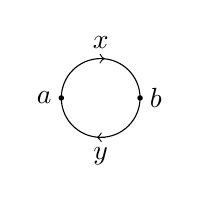
\begin{tikzpicture}[baseline=-4]
            \draw(0,0) circle[radius=0.5];
            \fill (-0.5,0) circle (1pt) node[left] {$a$};
            \fill (0.5,0) circle (1pt) node[right] {$b$};
            \node[above] at (0, 0.5) {$x$};
            \node[below] at (0, -0.5) {$y$};
            \draw[->] (-0.05, 0.5) -- (0.05, 0.5);
            \draw[<-] (-0.05, -0.5) -- (0.05, -0.5);
        \end{tikzpicture}

    Построим $C_0 = \Z a + \Z b$ --- свободная абелева группа на $\{a, b\}$, $C_1 = \Z x + \Z y$ --- тоже свободная абелева группа, но на образующих $\{x, y\}$.
        Вместо $\Z$ можно было взять любое другое кольцо.

    Все остальные элементы комплекса объявляются нулями.
    % https://q.uiver.app/#q=WzAsNCxbMCwwLCIwIl0sWzEsMCwiQ18xIl0sWzIsMCwiQ18wIl0sWzMsMCwiMCJdLFsyLDNdLFsxLDIsImRfMSJdLFswLDFdXQ==
        \[\begin{tikzcd}[ampersand replacement=\&]
              0 \& {C_1} \& {C_0} \& 0
              \arrow[from=1-3, to=1-4]
              \arrow["{d_1}", from=1-2, to=1-3]
              \arrow[from=1-1, to=1-2]
        \end{tikzcd}\]

    Определим $d_1$, как <<конец минус начало>>: $d_1(x) = b - a, d_1(y) = a - b$.

    Теперь $Z_0 = C_0, B_1 = 0, Z_1 = \Z(x + y), B_0 = \Z(b - a)$. Теперь $H_1 = Z_1/B_1 = \Z(x + y) \cong \Z$, и $H_0 = (\Z a + \Z b)/\Z(b - a) \cong \Z$
    \item Теперь триангулируем окружность по-другому:
        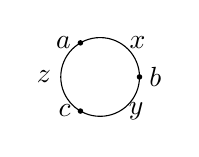
\begin{tikzpicture}[baseline=-4]
            \draw(0,0) circle[radius=0.5];
            \fill (-0.25,0.433) circle (1pt) node[left] {$a$};
            \fill (-0.25,-0.433) circle (1pt) node[left] {$c$};
            \fill (0.5,0) circle (1pt) node[right] {$b$};
            \node[above,right] at (0.25, 0.433) {$x$};
            \node[below,right] at (0.24, -0.433) {$y$};
            \node[left] at (-0.5, 0) {$z$};
        \end{tikzpicture} % todo стрелочки по касательной
    $d_1(x) = b - a, d_1(y) = c - b, d_1(z) = a - c$.

    Теперь $H_1 = Z_1 = \Z(x + y + z) \cong \Z$, и $B_0 = \Z(b + a)$, $B_0 = \Z(b - a) + \Z(c - b)$, и $H_0 = (\Z a + \Z b + \Z c)/ B_0 \cong \Z$.
    }
    Ответ получился тот же самый, и это не случайно --- есть такая теорема, что сингулярные/симплициальные гомологии (они равны для клеточных пространств) не зависят от триангуляции.
    \exercise{
    Триангулировать сферу, и вычислить гомологии.
    }
    Рассмотрим точную последовательность комплексов
    % https://q.uiver.app/#q=WzAsNSxbMCwwLCIwIl0sWzEsMCwiQSciXSxbMiwwLCJBIl0sWzMsMCwiQScnIl0sWzQsMCwiMCJdLFszLDRdLFsyLDNdLFsxLDJdLFswLDFdXQ==
    \[\begin{tikzcd}[ampersand replacement=\&]
          0 \& {A'} \& A \& {A''} \& 0
          \arrow[from=1-4, to=1-5]
          \arrow[from=1-3, to=1-4]
          \arrow[from=1-2, to=1-3]
          \arrow[from=1-1, to=1-2]
    \end{tikzcd}\]
    \theorem{
        Существует длинная точная последовательность гомологических групп
    % https://q.uiver.app/#q=WzAsNyxbMCwwLCJcXGNkb3RzIl0sWzEsMCwiSCciXSxbMiwwLCJIIl0sWzMsMCwiSCcnIl0sWzQsMCwiSCdbLTFdIl0sWzUsMCwiSFstMV0iXSxbNiwwLCJcXGNkb3RzIl0sWzAsMV0sWzEsMl0sWzIsM10sWzMsNF0sWzQsNV0sWzUsNl1d
        \[\begin{tikzcd}[ampersand replacement=\&]
              \cdots \& {H'} \& H \& {H''} \& {H'[-1]} \& {H[-1]} \& \cdots
              \arrow[from=1-1, to=1-2]
              \arrow[from=1-2, to=1-3]
              \arrow[from=1-3, to=1-4]
              \arrow[from=1-4, to=1-5]
              \arrow[from=1-5, to=1-6]
              \arrow[from=1-6, to=1-7]
        \end{tikzcd}\]
    где связующий морфизм $\delta$ будет построен в доказательстве.

    Более того, это всё функториально: если есть другая короткая точная последовательность, и морфизм между ними, то по отношению к ним найдётся естественный морфизм полученных длинных точных последовательностей гомологий.
    \provehere{
    Сначала строим $\delta$.

    Для $z \in Z_n''$, обозначим за $[z]$ класс $z$ в $H_n''$.
    % https://q.uiver.app/#q=WzAsMTAsWzAsMCwiMCJdLFsxLDAsIkFfbiciXSxbMiwwLCJBX24iXSxbMywwLCJBX24nJyJdLFs0LDAsIjAiXSxbMCwxLCIwIl0sWzEsMSwiQV97bi0xfSciXSxbMiwxLCJBX3tuLTF9Il0sWzMsMSwiQScnX3tuLTF9Il0sWzQsMSwiMCJdLFsyLDMsIlxccGkiXSxbMiw3LCJkIl0sWzYsNywiaSJdLFs3LDhdLFs4LDldLFszLDRdLFszLDgsImQnJyJdLFsxLDJdLFsxLDYsImQnIl0sWzAsMV0sWzUsNl1d
        \[\begin{tikzcd}[ampersand replacement=\&]
              0 \& {A_n'} \& {A_n} \& {A_n''} \& 0 \\
              0 \& {A_{n-1}'} \& {A_{n-1}} \& {A''_{n-1}} \& 0
              \arrow["\pi", from=1-3, to=1-4]
              \arrow["d", from=1-3, to=2-3]
              \arrow["i", from=2-2, to=2-3]
              \arrow[from=2-3, to=2-4]
              \arrow[from=2-4, to=2-5]
              \arrow[from=1-4, to=1-5]
              \arrow["{d''}", from=1-4, to=2-4]
              \arrow[from=1-2, to=1-3]
              \arrow["{d'}", from=1-2, to=2-2]
              \arrow[from=1-1, to=1-2]
              \arrow[from=2-1, to=2-2]
        \end{tikzcd}\]
    Положим $\delta([z]) \coloneqq [i^{-1}(d(\pi^{-1}(z)))]$, где $\pi^{-1}(z)$ --- произвольный прообраз (он есть, так как $\pi$ сюръективно).

            \comment{Дальше надо проверить, что определение корректно, и последовательность точна, но я не хочу это техать, доказательства не будет.}
    }
    }
\end{document}